%% LyX 2.2.2 created this file.  For more info, see http://www.lyx.org/.
%% Do not edit unless you really know what you are doing.
\documentclass[11pt,english]{beamer}
\usepackage{enumerate}

\usepackage{mathptmx}
\usepackage[T1]{fontenc}
\usepackage[utf8]{inputenc}
\setlength{\parskip}{\smallskipamount}
\setlength{\parindent}{0pt}
\usepackage{url}
\usepackage[authoryear]{natbib}
\usefonttheme[onlymath]{serif} % para las fuentes de las ecuaciones
\makeatletter
\usepackage{amsmath,amssymb,amsthm}
\usepackage{graphicx}
\usepackage{xcolor} % para colorear textos con \textcolor o \color
\usepackage{hyperref}
\usepackage{times}
\usepackage{array}
\usepackage{multicol}
\usepackage{longtable}
\usepackage{float} % para usar comando [H] en tablas y gr\'aficas
\usepackage{xcolor}% para modificar el color de la presentacion y del texto
\usepackage{colortbl} % para tablas de Kable
\usepackage{booktabs} % Para toprule: To thicken table lines 
\usepackage[nogin]{Sweave} % elimina el tamaño por default de las figuras de sweave
\usepackage{natbib}
\bibliographystyle{agsm}
% \usepackage[inline]{enumitem} % para enumerar dentro de un paragrafo
\usepackage{rotating} % para rotar nombres de columnas

\usepackage{graphicx}
\usepackage{subcaption}




%%%%%%%%%%%%%%%%%%%%%%%%%%%%%% LyX specific LaTeX commands.
\providecommand{\LyX}{L\kern-.1667em\lower.25em\hbox{Y}\kern-.125emX\@}

%%%%%%%%%%%%%%%%%%%%%%%%%%%%%% Textclass specific LaTeX commands.
 % this default might be overridden by plain title style
 \newcommand\makebeamertitle{\frame{\maketitle}}%
 % (ERT) argument for the TOC
 \AtBeginDocument{%
   \let\origtableofcontents=\tableofcontents
   \def\tableofcontents{\@ifnextchar[{\origtableofcontents}{\gobbletableofcontents}}
   \def\gobbletableofcontents#1{\origtableofcontents}
 }
\newcommand{\code}[1]{\texttt{#1}}

%%%%%%%%%%%%%%%%%%%%%%%%%%%%%% User specified LaTeX commands.
\usetheme{Warsaw}
% or ...

\setbeamercovered{transparent}
% or whatever (possibly just delete it)

\usepackage[T1]{fontenc}

\makeatother

% \usepackage{babel}
\usepackage{listings}
\renewcommand{\lstlistingname}{\inputencoding{latin9}Listing}

\begin{document}
\Sconcordance{concordance:2_medidas_descriptivas_multivariadas.tex:2_medidas_descriptivas_multivariadas.Rnw:1 %
49 1 1 4 144 1 1 10 37 0 1 2 1 1 1 7 29 1 1 6 1 5 15 0 1 2 32 1 2 4 36 %
0 1 2 25 1 2 4 15 0 1 2 14 1 1 4 1 5 16 0 1 2 61 1 1 9 21 0 1 2 103 1 1 %
6 1 2 4 1 1 8 1 2 5 1 1 8 1 2 7 1 1 12 1 2 121 1 1 35 14 0 1 4 22 1 1 6 %
1 24 14 0 1 2 62 1}



\title{Medidas descriptivas multivariadas}

\subtitle{Transcripción de las univariadas}

\author{Jimmy A Corzo S\inst{1} \inst{2}}

\institute[Profesor Titular]{\inst{1}Profesor Titular\\
Departamento de Estadística\and \inst{2}Facultad de ciencias\\
Universidad Nacional de colombia}

\date[2023]{Métodos multivariados aplicados \LyX{} cap 3}

\makebeamertitle

%\pgfdeclareimage[height=0.5cm]{institution-logo}{institution-logo-filename}

%\logo{\pgfuseimage{institution-logo}}

\AtBeginSubsection[]{

  \frame<beamer>{ 

    \frametitle{Outline}   

    \tableofcontents[currentsection,currentsubsection] 

  }

}

%\beamerdefaultoverlayspecification{<+->}
\begin{frame}
\tableofcontents{}
\end{frame}

\begin{frame}{Notación}
Para la construcción de los análogos multivariados de las medidas descriptivas univariadas primero se requiere definir las observaciones multivariadas.

En el contexto multivariado en lugar de una se observan $p$ variables $X_1,\ldots,X_p$ simultáneamente sobre mismo un objeto $i$ (que puede ser una ciudad, una universidad, una planta, una persona), y por tanto una observación para el objeto $i$ es un vector de $p$ componentes 
$$x_i = \left(x_{i1},\ldots,x_{ij},\ldots,x_{ip}\right)^\prime,$$
donde $x_{ij}$ es la observación de la variable $j$ sobre el objeto $i$. 
\end{frame}


\begin{frame}{tabla de datos}
Para $n$ objetos las observaciones se arreglan en una tabla de datos como la siguiente:
\begin{table}[H]
  \centering
  % \caption{Add caption}
    \begin{tabular}{ccccc}
           &            & Variables          &       & \\
    \toprule
    Objeto &     $ X_1$ &      $X_2$ &       &     $X_p$ \\
    \midrule
    1     & $x_{11}$ & $x_{12}$ & $\cdots$ & $x_{1p}$ \\
    $\vdots$ & $\vdots$ & $\vdots$ & $\vdots$ & $\vdots$ \\
    n     & $x_{n1}$ & $x_{n2}$ & $\cdots$ & $x_{np}$ \\
    \bottomrule
    \end{tabular}%
  \label{tab:addlabel}%
\end{table}%
\end{frame}

\begin{frame}{Media, Varianza, Covarianza y Coeficiente de correlación:}

\begin{align}\label{ec:descrpunivar}
\bar{x}_j&=\frac1n \sum_{i=1}^{n} x_{ij} \qquad \text{media de } X_j \notag \\
s_j^2&= \frac1n \sum_{i=1}^{n} (x_{ij}-\bar{x}_j)^2 \qquad \text{varianza de } X_j \notag \\
cov(X_j,X_k)&=s_{jk}=\frac1n \sum_{i=1}^{n} (x_{ij}-\bar{x}_j)(x_{ik}-\bar{x}_k), \quad\quad s_{jj} = s_j^2 \notag \\
corr(X_j,X_k)& = r_{jk}= \frac{s_{jk}}{s_j s_k}, \quad\quad s_j = \sqrt{s_j^2}
\end{align}
\end{frame}

\begin{frame}{tabla de datos}
\textbf{tabla} para referirse a los datos con nombres en las filas y columnas

\textbf{matriz} cundo se van a utilizar las propiedades algebraicas de la tabla

$$ X= \left\{x_{ij} \right\} = \left[ \begin{array}{cccc}
x_{11}& x_{12}& \cdots& x_{1p}\\
x_{21}& x_{22}& \cdots& x_{2p}\\
\vdots& \vdots& \vdots& \vdots\\
x_{n1}& x_{n2}& \cdots& x_{np}
\end{array} \right]$$
Se asume que $n\ge p$
\end{frame}

\begin{frame}{Columna de la tabla de datos}
En esta matriz la columna $j$, o el punto variable $j$, representa las observaciones de la variable $X_j$ sobre los $n$ objetos y se denota como un vector columna:
$$X_j= \left[ \begin{array}{c}
x_{1j}\\
x_{2j}\\
\vdots\\
x_{nj}\\
\end{array} \right], j=1,\ldots,p
$$
\end{frame}

\begin{frame}{Fila de la tabla de datos}
Análogamente, la fila $i$, o el punto objeto $i$, representa las observaciones de las $p$ variables sobre el objeto $i$ que se denota como un vector columna;
$$
x_i = \left(x_{i1},\ldots,x_{ip}\right)^\prime = \left[ \begin{array}{c}
x_{i1}\\
x_{i2}\\
\vdots\\
x_{ip}\\
\end{array} \right], i=1,\ldots,n.
$$
\end{frame}
% 
\begin{frame}{Vector de medias}
\begin{align}
\bar{x}=
\left[ \begin{array}{c}
\bar{x}_1\\
\bar{x}_2\\
\vdots\\
\bar{x}_p
\end{array} \right]
\end{align}
\end{frame}
% 
\begin{frame}[containsverbatim, allowframebreaks]{Ejemplo Ciudades Colombianas}

\setlength\abovecaptionskip{1pt}\begin{table}[!h]
\centering
\caption{\label{tab:CiuIndEdu}Tabla de datos multivariados de ciudades colombianas}
\centering
\resizebox{\ifdim\width>\linewidth\linewidth\else\width\fi}{!}{
\fontsize{6}{8}\selectfont
\begin{tabular}[t]{lrrrrr}
\toprule
  & Num.Hab & Analfabetismo & Cobertura.pria.y.secdaria & Cobertura.ed.sup & Rel.al.prof\\
\midrule
\cellcolor{gray!10}{Armenia} & \cellcolor{gray!10}{284120} & \cellcolor{gray!10}{0.09} & \cellcolor{gray!10}{1.09} & \cellcolor{gray!10}{0.27} & \cellcolor{gray!10}{22.4}\\
Barranquilla & 1163007 & 0.09 & 1.08 & 0.31 & 22.5\\
\cellcolor{gray!10}{Bogota} & \cellcolor{gray!10}{7050228} & \cellcolor{gray!10}{0.10} & \cellcolor{gray!10}{1.00} & \cellcolor{gray!10}{0.54} & \cellcolor{gray!10}{22.6}\\
Bucaramanga & 520080 & 0.08 & 1.19 & 0.33 & 22.2\\
\cellcolor{gray!10}{Cali} & \cellcolor{gray!10}{2169801} & \cellcolor{gray!10}{0.08} & \cellcolor{gray!10}{1.02} & \cellcolor{gray!10}{0.22} & \cellcolor{gray!10}{22.0}\\
\addlinespace
Cartagena & 912674 & 0.12 & 1.21 & 0.15 & 24.4\\
\cellcolor{gray!10}{Cucuta} & \cellcolor{gray!10}{600049} & \cellcolor{gray!10}{0.11} & \cellcolor{gray!10}{1.15} & \cellcolor{gray!10}{0.22} & \cellcolor{gray!10}{22.4}\\
Ibague & 509796 & 0.11 & 0.98 & 0.18 & 23.4\\
\cellcolor{gray!10}{Manizales} & \cellcolor{gray!10}{383483} & \cellcolor{gray!10}{0.08} & \cellcolor{gray!10}{1.14} & \cellcolor{gray!10}{0.23} & \cellcolor{gray!10}{22.2}\\
Medellin & 2264776 & 0.13 & 1.22 & 0.30 & 26.3\\
\addlinespace
\cellcolor{gray!10}{Monteria} & \cellcolor{gray!10}{390996} & \cellcolor{gray!10}{0.16} & \cellcolor{gray!10}{1.11} & \cellcolor{gray!10}{0.15} & \cellcolor{gray!10}{26.1}\\
Neiva & 322098 & 0.11 & 1.10 & 0.18 & 23.3\\
\cellcolor{gray!10}{Pasto} & \cellcolor{gray!10}{394074} & \cellcolor{gray!10}{0.11} & \cellcolor{gray!10}{1.05} & \cellcolor{gray!10}{0.13} & \cellcolor{gray!10}{21.8}\\
Pereira & 448971 & 0.10 & 1.12 & 0.28 & 22.6\\
\cellcolor{gray!10}{Popayan} & \cellcolor{gray!10}{261694} & \cellcolor{gray!10}{0.09} & \cellcolor{gray!10}{1.14} & \cellcolor{gray!10}{0.16} & \cellcolor{gray!10}{21.5}\\
\addlinespace
Riohacha & 184847 & 0.27 & 1.00 & 0.15 & 26.1\\
\cellcolor{gray!10}{San Andres} & \cellcolor{gray!10}{66675} & \cellcolor{gray!10}{0.08} & \cellcolor{gray!10}{0.80} & \cellcolor{gray!10}{0.11} & \cellcolor{gray!10}{20.4}\\
Santa Marta & 428374 & 0.12 & 1.00 & 0.12 & 22.9\\
\cellcolor{gray!10}{Sincelejo} & \cellcolor{gray!10}{245180} & \cellcolor{gray!10}{0.16} & \cellcolor{gray!10}{1.23} & \cellcolor{gray!10}{0.11} & \cellcolor{gray!10}{24.9}\\
Tunja & 161209 & 0.10 & 1.04 & 0.24 & 22.1\\
\addlinespace
\cellcolor{gray!10}{Valledupar} & \cellcolor{gray!10}{373872} & \cellcolor{gray!10}{0.16} & \cellcolor{gray!10}{1.02} & \cellcolor{gray!10}{0.15} & \cellcolor{gray!10}{24.5}\\
Villavicencio & 400475 & 0.10 & 1.19 & 0.17 & 25.4\\
\bottomrule
\end{tabular}}
\end{table}\end{frame}


\begin{frame}{FIla de la tabla de datos}
La fila 5 de la Tabla \ref{tab:CiuIndEdu} es la observación de las cinco variables para la ciudad de Cali (objeto 5):

$$x_{5}=(2169801, 0.08, 1.02, 0.22, 22)^\prime=
\left[ \begin{array}{c}
2168901\\
0.08\\
1.02\\
0.22\\
22\\
\end{array} \right]$$
\end{frame}

\begin{frame}{Columna de la tabla de datos}
la variable $X_4$ Cobertura en educación superior es la columna
$$X_4=\left[ \begin{array}{c}
0.27\\
0.31\\
\vdots\\
0.15\\
0.17\\
\end{array} \right]$$
\end{frame}

\section{Vector de medias, matriz de covarianzas y matriz de correlación}

% 
\begin{frame}{Ejemplo vector de meidas}
El vector de medias de las variables de la tabla de ciudades expresado como un vector es: $\bar{x}^\prime = (888021.77, 0.12, 1.09, 0.21, 23.27)^\prime$, el cual, en formato de tabla se muestra en la tabla\ref{tab:VecMedias} :

\begin{table}[!h]
\centering
\caption{\label{tab:VecMedias}Vector de medias para variables de educación 
      de la tabla de ciudades}
\centering
\begin{tabular}[t]{lr}
\toprule
  & Media\\
\midrule
\cellcolor{gray!10}{Num.Hab} & \cellcolor{gray!10}{888021.77}\\
Analfabetismo & 0.12\\
\cellcolor{gray!10}{Cobertura.pria.y.secdaria} & \cellcolor{gray!10}{1.09}\\
Cobertura.ed.sup & 0.21\\
\cellcolor{gray!10}{Rel.al.prof} & \cellcolor{gray!10}{23.27}\\
\bottomrule
\end{tabular}
\end{table}\end{frame}

\begin{frame}{Matriz de datos centrados}
Contiene las observaciones centradas estandarizados\vskip1mm
$$y_{ij}  = \frac{x_{ij}- \bar{x}_j}{s_j} $$:

$$ Y = \left\{y_{ij} \right\} = 
\frac{x_{ij}- \bar{x}_j}{s_j} = \left[ \begin{array}{cccc}

\frac{x_{11}-\bar{x}_1}{s_1} & \frac{x_{12}-\bar{x}_2}{s_2} & \cdots &\frac{x_{1p}-\bar{x}_p}{s_p} \\
\frac{x_{21}-\bar{x}_1}{s_1} & \frac{x_{22}-\bar{x}_2}{s_2} & \cdots &\frac{x_{2p}-\bar{x}_p}{s_P}\\
\vdots& \vdots               & \vdots& \vdots\\
\frac{x_{n1}-\bar{x}_1}{s_1} & \frac{x_{n2}-\bar{x}_2}{s_2} & \cdots& \frac{x_{np}-\bar{x}_p}{s_p}
\end{array} \right]$$

de manera que $med(\bar{Y_j}) = 0$ y $var(Y_j) = 1$
\end{frame}
% 
% \begin{frame}{Matriz de datos centrados y estandarizados}
% contiene las observaciones centradas y estandarizadas $\widetilde{x}_{ij}^*  = (x_{ij}- \bar{x}_j)/s_j$:
% $$ \widetilde{X}^* = \left\{\widetilde{x}_{ij}^* \right\}  = \left[ \begin{array}{cccc}
% \widetilde{x}_{11}^* & \widetilde{x}_{12}^* & \cdots & \widetilde{x}_{1p}^*\\
% \widetilde{x}_{21}^* & \widetilde{x}_{22}^* & \cdots & \widetilde{x}_{2p}^*\\
% \vdots& \vdots & \vdots& \vdots\\
% \widetilde{x}_{n1}^* & \widetilde{x}_{12}^* & \cdots & \widetilde{x}_{np}^*
% \end{array} \right]$$
% de manera que $var(\widetilde{x}_{j}^*) = 1) $
% \end{frame}
% % 
\begin{frame}[containsverbatim, allowframebreaks]
\frametitle{Matriz de datos centrados}
Se puede comprobar fácilmente que todas las variables tienen media cero.


\begin{table}[!h]
\centering
\caption{\label{tab:DatosCent}Matriz de datos centrados}
\centering
\resizebox{\ifdim\width>\linewidth\linewidth\else\width\fi}{!}{
\begin{tabular}[t]{lrrrrr}
\toprule
  & Num.Hab & Analfabetismo & Cobertura.pria.y.secdaria & Cobertura.ed.sup & Rel.al.prof\\
\midrule
\cellcolor{gray!10}{Armenia} & \cellcolor{gray!10}{-603901.77} & \cellcolor{gray!10}{-0.028} & \cellcolor{gray!10}{0.009} & \cellcolor{gray!10}{0.053} & \cellcolor{gray!10}{-0.873}\\
Barranquilla & 274985.23 & -0.024 & -0.003 & 0.093 & -0.773\\
\cellcolor{gray!10}{Bogota} & \cellcolor{gray!10}{6162206.23} & \cellcolor{gray!10}{-0.019} & \cellcolor{gray!10}{-0.087} & \cellcolor{gray!10}{0.325} & \cellcolor{gray!10}{-0.673}\\
Bucaramanga & -367941.77 & -0.040 & 0.106 & 0.113 & -1.073\\
\cellcolor{gray!10}{Cali} & \cellcolor{gray!10}{1281779.23} & \cellcolor{gray!10}{-0.033} & \cellcolor{gray!10}{-0.067} & \cellcolor{gray!10}{0.010} & \cellcolor{gray!10}{-1.273}\\
\addlinespace
Cartagena & 24652.23 & 0.005 & 0.121 & -0.066 & 1.127\\
\cellcolor{gray!10}{Cucuta} & \cellcolor{gray!10}{-287972.77} & \cellcolor{gray!10}{-0.003} & \cellcolor{gray!10}{0.061} & \cellcolor{gray!10}{0.004} & \cellcolor{gray!10}{-0.873}\\
Ibague & -378225.77 & -0.009 & -0.103 & -0.032 & 0.127\\
\cellcolor{gray!10}{Manizales} & \cellcolor{gray!10}{-504538.77} & \cellcolor{gray!10}{-0.039} & \cellcolor{gray!10}{0.057} & \cellcolor{gray!10}{0.017} & \cellcolor{gray!10}{-1.073}\\
Medellin & 1376754.23 & 0.010 & 0.133 & 0.087 & 3.027\\
\addlinespace
\cellcolor{gray!10}{Monteria} & \cellcolor{gray!10}{-497025.77} & \cellcolor{gray!10}{0.043} & \cellcolor{gray!10}{0.023} & \cellcolor{gray!10}{-0.062} & \cellcolor{gray!10}{2.827}\\
Neiva & -565923.77 & -0.003 & 0.014 & -0.034 & 0.027\\
\cellcolor{gray!10}{Pasto} & \cellcolor{gray!10}{-493947.77} & \cellcolor{gray!10}{-0.005} & \cellcolor{gray!10}{-0.034} & \cellcolor{gray!10}{-0.085} & \cellcolor{gray!10}{-1.473}\\
Pereira & -439050.77 & -0.015 & 0.038 & 0.070 & -0.673\\
\cellcolor{gray!10}{Popayan} & \cellcolor{gray!10}{-626327.77} & \cellcolor{gray!10}{-0.025} & \cellcolor{gray!10}{0.049} & \cellcolor{gray!10}{-0.050} & \cellcolor{gray!10}{-1.773}\\
\addlinespace
Riohacha & -703174.77 & 0.155 & -0.086 & -0.061 & 2.827\\
\cellcolor{gray!10}{San Andres} & \cellcolor{gray!10}{-821346.77} & \cellcolor{gray!10}{-0.039} & \cellcolor{gray!10}{-0.283} & \cellcolor{gray!10}{-0.106} & \cellcolor{gray!10}{-2.873}\\
Santa Marta & -459647.77 & 0.008 & -0.081 & -0.097 & -0.373\\
\cellcolor{gray!10}{Sincelejo} & \cellcolor{gray!10}{-642841.77} & \cellcolor{gray!10}{0.045} & \cellcolor{gray!10}{0.142} & \cellcolor{gray!10}{-0.106} & \cellcolor{gray!10}{1.627}\\
Tunja & -726812.77 & -0.014 & -0.050 & 0.032 & -1.173\\
\addlinespace
\cellcolor{gray!10}{Valledupar} & \cellcolor{gray!10}{-514149.77} & \cellcolor{gray!10}{0.043} & \cellcolor{gray!10}{-0.069} & \cellcolor{gray!10}{-0.066} & \cellcolor{gray!10}{1.227}\\
Villavicencio & -487546.77 & -0.014 & 0.107 & -0.039 & 2.127\\
\bottomrule
\end{tabular}}
\end{table}\end{frame}

\begin{frame}{Matriz de covarianzas}
Es una matriz simétrica que contiene en su diagonal las varianzas de las variables  $s_j^2$, y por fuera de la diagonal las covarianzas $s_{jk}$ entre ellas.

$$ S =  \left[ \begin{array}{cccc}
s_1^2& s_{12}& \cdots& s_{1p}\\
s_{21}& s_2^2& \cdots& s_{2p}\\
\vdots& \vdots& \vdots& \vdots\\
s_{p1}& s_{p2}& \cdots& s_p^2
\end{array} \right], \quad s_j^2 = s_{jj} $$
\end{frame}

\begin{frame}{Otras medidas de variabilidad multivariada}


\textbf{Varianza generalizada} definida como el determinante de la matriz de covarianzas $|S|$\\

\textbf{Varianza total} definida como $Traza(S)$\\
%  o como $Traza(R)$, $R$ matriz de correlación
Éstas se pueden expresar en términos de los valores propios de $S$, los cuales como se verá más adelante, son las varianzas de las componentes principales (factores).
\end{frame}

\begin{frame}{Ejemplo}
Matriz de covarianzas entre las variables del archivo de ciudades.


\begin{table}[!h]
\centering
\caption{\label{tab:MatCov}Matriz de covarianzas de las variables del archivo de ciudades}
\centering
\resizebox{\ifdim\width>\linewidth\linewidth\else\width\fi}{!}{
\begin{tabular}[t]{lrrrrr}
\toprule
  & Num.Hab & Analfabetismo & Cobertura.pria.y.secdaria & Cobertura.ed.sup & Rel.al.prof\\
\midrule
\cellcolor{gray!10}{Num.Hab} & \cellcolor{gray!10}{2.228013e+12} & \cellcolor{gray!10}{-9797.725} & \cellcolor{gray!10}{-13331.063} & \cellcolor{gray!10}{116811.812} & \cellcolor{gray!10}{-34962.921}\\
Analfabetismo & -9.797725e+03 & 0.002 & 0.000 & -0.001 & 0.050\\
\cellcolor{gray!10}{Cobertura.pria.y.secdaria} & \cellcolor{gray!10}{-1.333106e+04} & \cellcolor{gray!10}{0.000} & \cellcolor{gray!10}{0.010} & \cellcolor{gray!10}{0.001} & \cellcolor{gray!10}{0.070}\\
Cobertura.ed.sup & 1.168118e+05 & -0.001 & 0.001 & 0.010 & -0.025\\
\cellcolor{gray!10}{Rel.al.prof} & \cellcolor{gray!10}{-3.496292e+04} & \cellcolor{gray!10}{0.050} & \cellcolor{gray!10}{0.070} & \cellcolor{gray!10}{-0.025} & \cellcolor{gray!10}{2.721}\\
\bottomrule
\end{tabular}}
\end{table}\end{frame}

\begin{frame}{Matriz de correlación}
Es una matriz simétrica que contiene unos en la diagonal que son las correlaciones de las variables consigo mismas y por fuera de la diagonal las correlaciones $r_{ij}$ entre pares de variables.

$$ R =  \left[ \begin{array}{cccc}
   1  & r_{12}& \cdots& r_{1p}\\
r_{21}&    1  & \cdots& r_{2p}\\
\vdots& \vdots& \vdots& \vdots\\
r_{p1}& r_{p2}& \cdots&    1
\end{array} \right], \quad r_{ij}=\frac{s_{ij}}{s_is_j} $$
\end{frame}

\begin{frame}{Ejemplo}
Matriz correlación entre las variables de la tabla de ciudades.

\begin{table}[!h]
\centering
\caption{\label{tab:MatCor}Matriz de correlación de las variables 
      del archivo de ciudades}
\centering
\resizebox{\ifdim\width>\linewidth\linewidth\else\width\fi}{!}{
\begin{tabular}[t]{lrrrrr}
\toprule
  & Num.Hab & Analfabetismo & Cobertura.pria.y.secdaria & Cobertura.ed.sup & Rel.al.prof\\
\midrule
\cellcolor{gray!10}{Num.Hab} & \cellcolor{gray!10}{1.00} & \cellcolor{gray!10}{-0.15} & \cellcolor{gray!10}{-0.09} & \cellcolor{gray!10}{0.79} & \cellcolor{gray!10}{-0.01}\\
Analfabetismo & -0.15 & 1.00 & -0.01 & -0.34 & 0.71\\
\cellcolor{gray!10}{Cobertura.pria.y.secdaria} & \cellcolor{gray!10}{-0.09} & \cellcolor{gray!10}{-0.01} & \cellcolor{gray!10}{1.00} & \cellcolor{gray!10}{0.09} & \cellcolor{gray!10}{0.42}\\
Cobertura.ed.sup & 0.79 & -0.34 & 0.09 & 1.00 & -0.15\\
\cellcolor{gray!10}{Rel.al.prof} & \cellcolor{gray!10}{-0.01} & \cellcolor{gray!10}{0.71} & \cellcolor{gray!10}{0.42} & \cellcolor{gray!10}{-0.15} & \cellcolor{gray!10}{1.00}\\
\bottomrule
\end{tabular}}
\end{table}\end{frame}

\begin{frame}{Combinaciones lineales}
Una combinación lineal es una suma ponderada de los valores de una variable observada en varios objetos, como lo es la media por ser la suma de los valores de la variable ponderados por $1/n$, o como la varianza que es la suma de los desvíos de los valores de la variable respecto a la media $(x_i-\bar{x})^2$ poderados por $1/n$.
\end{frame}

\begin{frame}{Combinaciones lineales}
También es combinación lineal la una suma ponderada de los valores de varias variables observadas en un mismo objeto. Por ejemplo:
\vskip1mm
Los rankings de universidades
\vskip1mm
El índice de pobreza multidimensional es una combinación lineal de indicadores de vivienda, servicios básicos, estándar de vida, educación y empleo, y protección social; 
\vskip1mm
el índice de desarrollo humano que podera indicadores de dimensiones como la esperanza de vida, educación y riqueza. \vskip1mm
la mayoría de los índices o indicadores utilizados en economía y finanzas para describir y comparar cantidades de diferente naturaleza.
\end{frame}

\begin{frame}{Combinaciones lineales}
Las combinaciones lineales son útiles en muchos contextos estadísticos y especialmente en el caso de datos multivariados, donde por ejemplo, \textcolor{blue}{las componentes principales son combinaciones lineales de los valores de las variables cuyas ponderaciones se construyen para que contengan la mayor cantidad  posible de la varianza de las variables.}
\end{frame}

\begin{frame}{Combinación lineal de los valores de una variable observada en $n$ objetos}
Para la variable cuyas observaciones están en la columna  $j$ de la matriz de datos se define la combinación de los $n$ valores de la variable con constantes de ponderación $a^\prime = (a_1,\ldots,a_n)$ por:
\begin{eqnarray}\label{CLineal}\label{ec:CoLin}
X^\star_j = \sum_{i=1}^n a_ix_{ij}   \ \ \  j=1,\ldots,p \quad \text{vectorialmente} \quad (a^\prime X_j)
\end{eqnarray}
\end{frame}

\begin{frame}{Ejemplo}
En particular, el promedio de la variable $j$ es una combinación lineal con constantes de ponderación $p^\prime = (\frac1n,\ldots,\frac1n)$:
$$
\bar{x}_j = \sum_{i=1}^n \frac1n x_{ij}  \quad \text{vectorialmente} \quad (p^\prime X_j)
$$.
\end{frame}

\begin{frame}{Combinación lineal de valores de $p$ variables observadas sobre un mismo objeto}
Para el objeto $i$ de la matriz de datos, cuyas observaciones están en la fila $x_i^\prime = \left(x_{i1},\ldots,x_{ip}\right)^\prime $ de la matriz de datos, se define la  combinación lineal de los valores de las $p$ variables con ponderaciones $b^\prime = (b_1,\ldots,b_p)$ por:

\begin{eqnarray}\label{CLineal}\label{ec:CoLin}
z_i = \sum_{j=1}^p b_jx_{ij}   \ \ \  i=1,\ldots,n, \quad \text{vectorialmente} \quad (b^\prime x_i)
\end{eqnarray}

Conviene aclarar que este tipo de combinaciones lineales solo tienen sentido si las variables están estandarizadas, o cuando todas vienen medidas en las mismas escalas.
\end{frame}

\begin{frame}[containsverbatim, allowframebreaks]
\frametitle{Ejemplo. El Academic Rank of World Universities}

Uno de los más exigentes rankings del mundo es el Academic Rank of World Universities (ARWU) que utiliza los siguientes seis criterios de actividad académica e investigativa de las universidades (en paréntesis las pondetaciones de cada criterio)
\begin{itemize}
	\item \small  Premios Nobel de exalumnos (Score on Alumni: $X_1$) (10\%)
	\item \small  Premios Nobel de docentes de la universidad (Score on Award: $X_2$) (20\%)
	\item \small  Artículos altamente citados en 21 categor?as tem?ticas (Score on HiCi: $X_3$) (20\%)
	\item \small  Artículos publicados en las reconocidas revistas Nature y Science (Score on N\&S: $X_4$) (20\%) 
	\item \small  Artículos indexados en alguno de los índices de citación como el Science Citation Index-expanded o en el Social Science Citation Index (Score on PUB: $X_5$) (20\%) 
	\item \small  Productividad per cápita de los docentes de la universidad (Score on PCP: $X_6$) (10\%)
\end{itemize}
\end{frame}

\begin{frame}[containsverbatim, allowframebreaks]
\frametitle{Ejemplo. El Academic Rank of World Universities}
Los valores de los rankings para las primeras 10 universidades en el año 2013 se muestran en la  tabla \ref{tab:RankArwu}:
\begin{table}[!h]
\centering
\caption{\label{tab:RankArwu}Puntajes de las diez primeras universidades del ARWU}
\centering
\resizebox{\ifdim\width>\linewidth\linewidth\else\width\fi}{!}{
\begin{tabular}[t]{lrrrrrrr}
\toprule
  & Alumni & Award & HiCi & N.S & PUB & PCP & Total.Score\\
\midrule
\cellcolor{gray!10}{Harvard} & \cellcolor{gray!10}{100.0} & \cellcolor{gray!10}{100.0} & \cellcolor{gray!10}{100.0} & \cellcolor{gray!10}{100.0} & \cellcolor{gray!10}{100.0} & \cellcolor{gray!10}{69.2} & \cellcolor{gray!10}{100.0}\\
California, Berkeley & 67.6 & 79.3 & 69.0 & 70.9 & 70.6 & 54.2 & 72.4\\
\cellcolor{gray!10}{Stanford} & \cellcolor{gray!10}{40.2} & \cellcolor{gray!10}{78.4} & \cellcolor{gray!10}{87.6} & \cellcolor{gray!10}{68.4} & \cellcolor{gray!10}{69.7} & \cellcolor{gray!10}{50.1} & \cellcolor{gray!10}{72.1}\\
MIT & 70.5 & 80.3 & 66.8 & 70.1 & 61.4 & 64.5 & 71.4\\
\cellcolor{gray!10}{Cambridge} & \cellcolor{gray!10}{88.5} & \cellcolor{gray!10}{92.6} & \cellcolor{gray!10}{53.9} & \cellcolor{gray!10}{54.3} & \cellcolor{gray!10}{65.7} & \cellcolor{gray!10}{53.1} & \cellcolor{gray!10}{69.6}\\
\addlinespace
California I of Tech & 50.3 & 68.8 & 56.7 & 64.8 & 46.9 & 100.0 & 64.4\\
\cellcolor{gray!10}{Princeton} & \cellcolor{gray!10}{56.4} & \cellcolor{gray!10}{84.8} & \cellcolor{gray!10}{61.1} & \cellcolor{gray!10}{43.3} & \cellcolor{gray!10}{44.3} & \cellcolor{gray!10}{65.5} & \cellcolor{gray!10}{60.8}\\
Columbia & 70.7 & 67.4 & 56.2 & 47.6 & 69.9 & 32.1 & 60.4\\
\cellcolor{gray!10}{Chicago} & \cellcolor{gray!10}{65.5} & \cellcolor{gray!10}{83.9} & \cellcolor{gray!10}{50.9} & \cellcolor{gray!10}{39.8} & \cellcolor{gray!10}{50.5} & \cellcolor{gray!10}{40.0} & \cellcolor{gray!10}{57.3}\\
Oxford & 56.2 & 57.6 & 48.8 & 49.8 & 68.5 & 41.1 & 56.4\\
\bottomrule
\end{tabular}}
\end{table}\end{frame}

\begin{frame}{Ejemplo. El Academic Rank of World Universities}
El puntaje del ranking es una combinación lineal de los puntajes obtenidos por una universidad en los criterios, con ponderaciones $b^\prime = (0.1, 0.2, 0.2, 0.2, 0.2, 0.1) $, de manera que por ejemplo para la universidad de Harvard, cuyos puntajes en los criterios que están en la fila uno de la  tabla \ref{tab:RankArwu} son  \vskip1mm
$x_1=$(100, 100, 100, 100, 100, 69.2),\vskip1mm 
de manera que el valor de su  puntaje total en el ranking es:
\begin{align*}
	y_i&=0.1\times 100+0.2\times 100+0.2\times 100+0.2\times 100+0.2\times 100\\
	& +0.1\times 69.2=0.9692
\end{align*}
Ajustado a 100 en la tabla como máximo valor de referencia. 
\end{frame}

\begin{frame}{Ejemplo. El Academic Rank of World Universities}
Esto significa que para obtener los valores de la tabla hay que ajustar los valores que produce la combinación lineal. Por ejemplo, para la universidad de Cambridge:
\begin{align*}
	x_5&=0.1\times 88.5+ 0.2\times 92.6 +0.2\times 53.9 + 0.2\times 54.3 + 0.2\times 65.7\\
	& + 0.1\times 53.1= 0.6746
\end{align*}
% <<>>=
% 0.1* 88.5+ 0.2* 92.6 +0.2* 53.9 + 0.2* 54.3 + 0.2* 65.7 + 0.1* 53.1
% @


y por tanto después de ajustado $67.46/0.9692=69.6$.
\end{frame}

\begin{frame}{Componentes principales: Combinaciones lineales de las variables}
Propiedades:

\begin{itemize}
	\item [--] Van en direcciones que acumulan la mayor cantidad posible de varianza de la tabla de datos $X$: Util para reducir la dimensionalidad
	\item [--] Son independientes entre sí: facilita hacer representaciones gráficas de los datos.
\end{itemize}
\end{frame}

\begin{frame}{Componentes principales: Construcción}
Asumiendo que los datos están centrados y estandarizados $y_{ij} = (x_{ij} - \bar{x_j})/s_j$. 
\vskip1mm
Se utilizan unas ponderaciones $u_1^\prime = (u_{11}, \ldots, u_{p1}) $ tales que por ejemplo la primera componente es un conjunto de  $n$ puntos objeto (fila) de la forma:
\begin{equation}\label{primeraCP}
	z_{i1} = u_{11}y_{i1} + u_{21}y_{i2} + \cdots + u_{p1}y_{ip}
	= \sum_{j=1}^p u_{j1}y_{ij}, \qquad i=1,\dots,n,
\end{equation}
de manera que cada uno de los $n$ puntos es una especie de promedio ponderado de las variables observadas para cada objeto.
\end{frame}
%
\begin{frame}{Componentes principales 1: Teorema de la descomposición espectral (\textbf{TDE})}
Este teorema garantiza que una matriz simétrica $B_{p\times p} $ (generalmente la matriz de correlación $R$ o la matriz de covarianzas $S$) se puede reconstruir (o factorizar) a partir de sus \textbf{valores} y \textbf{vectores propios} como sigue:
\begin{equation}\label{TDespectr}
B=U\Lambda U^\prime
\end{equation}
$U$ es una \textbf{matriz ortogonal cuyas columnas son los vectores propios estandarizados de} $B$\vskip1mm
$\Lambda= diag\{\lambda_\alpha\}$ con $\lambda_1 \ge \cdots\ge\lambda_p$ son los \textbf{valores propios de}  $B$ arreglados en forma descendente.
(\cite{MardiaKentBibby}), p. 469).
\end{frame}
%
\begin{frame}{Componentes principales 2: Teorema de la descomposición espectral (\textbf{TDE})}
En particular cuando $B=R$ que es el caso más común
\begin{equation}\label{TDespectr1}\notag
R=U\Lambda U^\prime,
\end{equation}
$U$ contiene en sus columnas los vectores propios de $R$ y en la diagonal de $\Lambda$ están los valores propios de $R$.\vskip1mm 
Entonces la multiplicación de cada columna de $U$ por cada fila de la matriz de datos centrada y estandarizada $Y$ produce una componente principal del tipo (\ref{primeraCP}).

Cuando cuando $B=S$ es la matriz de covarianzas que es un caso menos común
\begin{equation}\label{TDespectr1}\notag
S=U\Lambda U^\prime,
\end{equation}
$U$ contiene los vectores propios de $S$  y $\Lambda$ contiene los valores propios de $S$
\end{frame}
%
\begin{frame}
Entonces tomando la $j$-ésima columna de $U$ denotada por $u_j^\prime = (u_{1j},\ldots, u_{pj})^\prime$, la $j$-ésima componente principal se obtiene como el producto: 
% \textcolor{red}{ revisar manejo de subíndices}:
\begin{align}
Y u_j =
\left[ \begin{array}{c}
\sum_{k=1}^{p}u_{kj}y_{1k} \\
\vdots\\
\sum_{k=1}^{p}u_{kj}y_{ik} \\
\vdots\\
\sum_{k=1}^{p}u_{kj}y_{nk} 
\end{array} \right]
= \left[ \begin{array}{c}
z_{11} \\
\vdots\\
z_{ij} \\
\vdots\\
z_{np}  
\end{array} \right], \quad j=1,\ldots,p
\end{align}
y para $j=1$ corresponde a \ref{primeraCP}.
\end{frame}
%
\begin{frame}{allowframebreaks}
\frametitle{Ejemplo RankinG ARWU}
Aunque en la práctica no se justifica ACP con dos variables puesto que el coeficiente de correlación y una gráfica de los puntos bastan para encontrar y representar las relaciones entre ellas, se realiza un PCA de los ranking regional y mundial con el único objetivo de ilustrar cómo funcionan las componentes y el tipo de información que contienen
\end{frame}

\begin{frame}{Ejemplo RankinG ARWU}
\setkeys{Gin}{width=0.8\textwidth} % redefinir el tamaño graficos
\begin{figure}[H]
	\centering
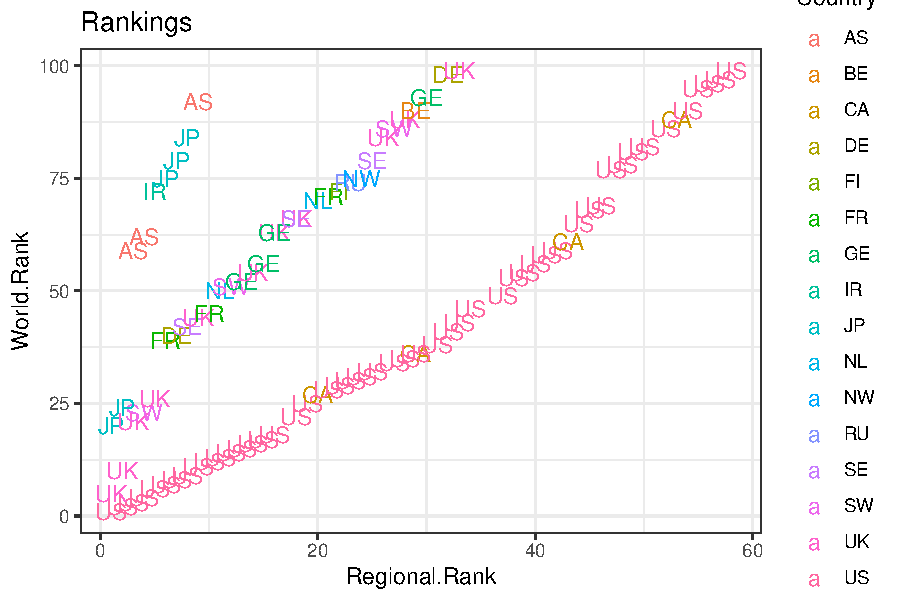
\includegraphics{2_medidas_descriptivas_multivariadas-013}
	\caption{Arwu...}\label{fig:arwuRegWorl}
\end{figure}
\end{frame}

\begin{frame}{Ejemplo RankinG ARWU}
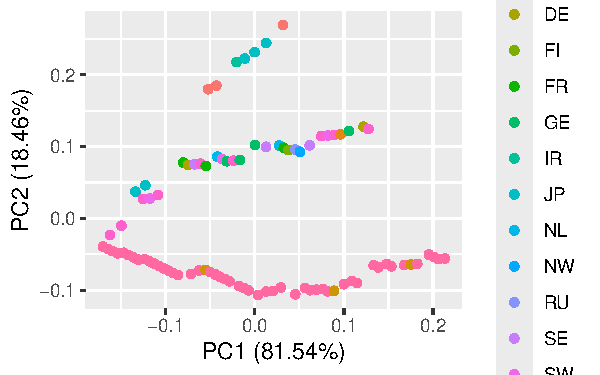
\includegraphics{2_medidas_descriptivas_multivariadas-014}
\end{frame}
% 
\begin{frame}{Ejemplo Ciudades}
\setkeys{Gin}{width=0.7\textwidth} % redefinir el tamaño graficos
\begin{figure}[H]
	\centering
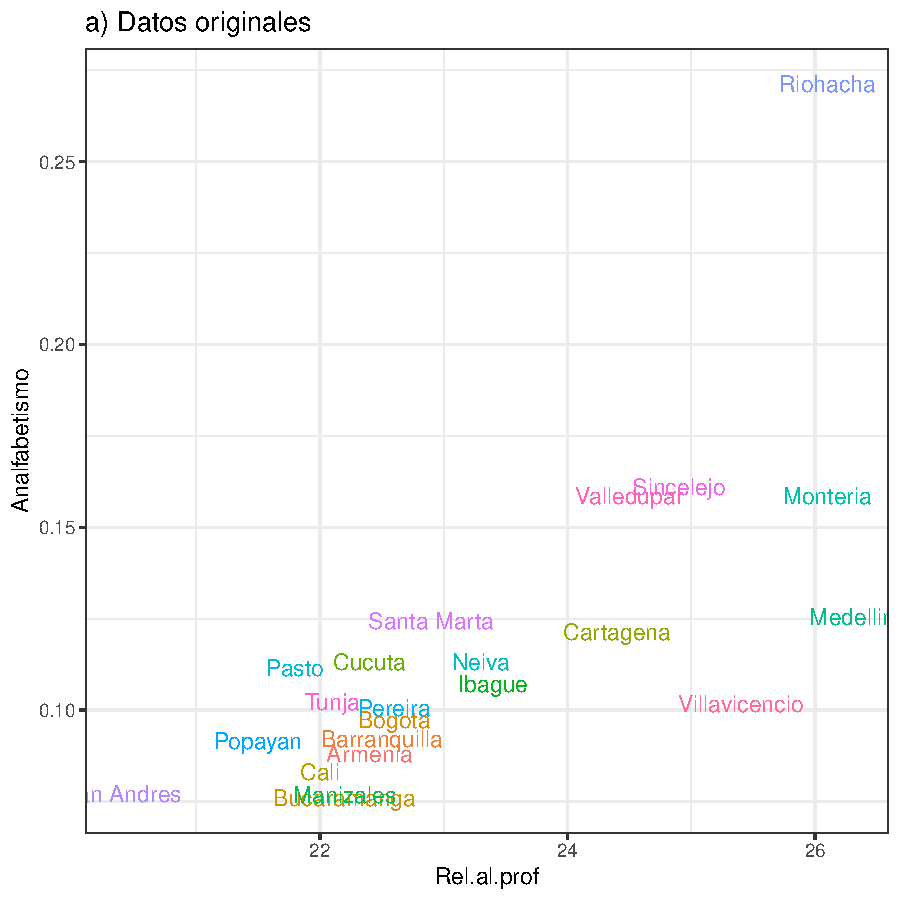
\includegraphics{2_medidas_descriptivas_multivariadas-015}
	\caption{Ciudades}\label{fig:idiCiudadesl}
\end{figure}
\end{frame}
% 
\begin{frame}{Ejemplo Ciudades}
\setkeys{Gin}{width=0.7\textwidth} % redefinir el tamaño graficos
\begin{figure}[H]
	\centering
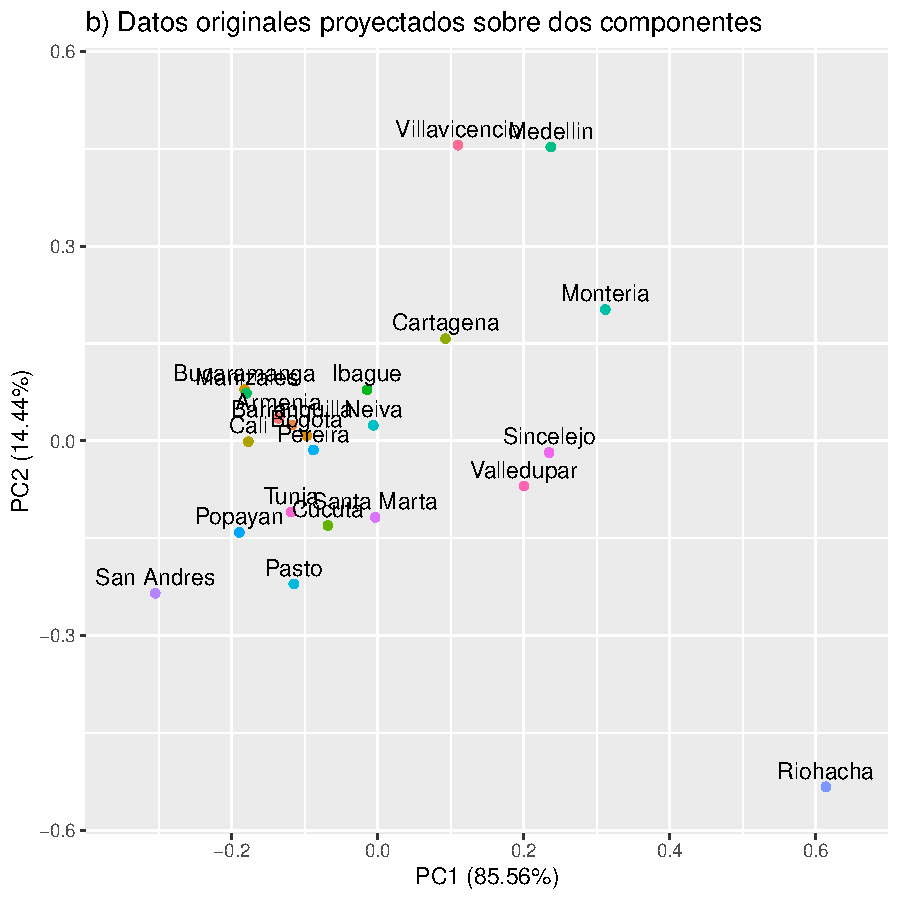
\includegraphics{2_medidas_descriptivas_multivariadas-016}
	\caption{Ciudades}\label{fig:idiCiudadesl}
\end{figure}
\end{frame}
% 
% \begin{frame}{   }
% \setkeys{Gin}{width=1\textwidth} % redefinir el tamaño graficos
% \begin{figure}[H]
% 	\centering
% <<fig=T, echo=F, height=4, width=8>>=
% df <- ciudades[,c(6,4)]
% # df <- arwu[1:20,4:5]
% pca_res_ciu <- prcomp(df, scale. = TRUE)
% 
% # autoplot(pca_res)
% autoplot(pca_res_ciu, data = ciudades, colour = "CIUDADES")
% @
% 	\caption{PCA }\label{fig:idiCiudades2}
% \end{figure}
% \end{frame}

% \begin{frame}{   }
% \setkeys{Gin}{width=1\textwidth} % redefinir el tamaño graficos
% \begin{figure}[H]
% 	\centering
% <<fig=T, echo=F, height=7, width=10>>=
% df <- ciudades[,c(6,3)]
% rownames(df) <- ciudades$CIUDADES
% pca_res_ciu <- prcomp(df, scale. = TRUE)
% biplot(pca_res_ciu, scale = 0)
% @
% 	\caption{Representación simultánea sobre los dos primeros factores}\label{fig:VrSObrefactores1}
% \end{figure}
% \end{frame}

% <<echo=F>>=
% # ciudades<-read.csv2("G:/Mi unidad/1- multivariado aplicado 2023/Multivariado I 2024 Diapositivas/Archivos para diapositivas/ciudades.csv", sep=";")
% X1<-as.matrix(ciudades[,c(3,6)])
% y<-scale(X1)    # matriz de datos estandarizada
%                 # Matriz de correlación a partir de la matriz de
%                 #  datos estandarizados Ry
% Ry<-(1/(nrow(y)-1))*t(y)%*%y
% eiY<-eigen(Ry)  # C?lculo de val. y vec. propios de Ry
%                 # C?lculo de las dos componentes principales
% cp<-(1/sqrt(nrow(y)))*y%*%eiY$vectors
% @
% ___________________________________________________________
% \begin{frame}
% \setkeys{Gin}{width=0.6\textwidth} % redefinir el tamaño graficos
% \begin{figure}[H]
% 	\centering
% <<fig=T, echo=F>>=
% X1<-as.matrix(ciudades[,c(3,6)])
% y<-scale(X1)    # matriz de datos estandarizada
%                 # Matriz de correlación a partir de la matriz de
%                 #  datos estandarizados Ry
% Ry<-(1/(nrow(y)-1))*t(y)%*%y
% eiY<-eigen(Ry)  # C?lculo de val. y vec. propios de Ry
%                 # C?lculo de las dos componentes principales
% cp<-(1/sqrt(nrow(y)))*y%*%eiY$vectors
% library(PlaneGeometry) # Para la función draw y otras más
% require(stats) # para el abline
% require(graphics) # para el abline
% X1<-as.matrix(ciudades[,c(3,6)])
% rownames(X1)<-ciudades$CIUDADES
% regresion=lm(X1[,1] ~ X1[,2])
% par(mfrow=c(2,2), mai = c(0,0.1,0.1,0.1))
% 
% plot(X1[,2], X1[,1], xlab = "Relación alumno-profesor",
%      ylab = "Analfabetismo",
%      main = "A.", xlim=c(20,27), ylim = c(0,0.3))
% abline(regresion, col = "red")
% grid()
% text(X1[,2], X1[,1], row.names(X1), cex = 0.7, col = "blue", pos = 1)
% l2 <- Line$new(c(23,0.2), c(24.5,0.06), FALSE, FALSE)
% draw(l2, col = "red", lwd = 1)
% 
% plot(cp[,1],cp[,2], xlab = "Factor 1", ylab = "Factor 2",
%      main = "B. ", xlim = c(-0.5, 0.9), ylim = c(-0.4,0.3))
% text(cp[,1],cp[,2], row.names(X1), cex = 0.7, pos = 3, col = "blue")
% abline(h = 0, v = 0, col = "red")
% @
% 	\caption{A: Coordenadas originales de las variables. B: componentes principales}\label{fig:VrOriginales}
% \end{figure}
% \end{frame}
% ___________________________________________________________________


\begin{frame}[containsverbatim, allowframebreaks]
\frametitle{Distancias entre observaciones multivariadas}
Intuitivamente la distancia entre dos puntos A y B en una superficie plana es la longitud del espacio que hay enre ellos. Entonces si se desea ir de A hacia B la distancia se puede medir en metros y esto da idea de lo lejos (o cerca) que están.
\end{frame}

\begin{frame}[containsverbatim, allowframebreaks]
\frametitle{Distancias o métricas entre observaciones multivariadas}
Esta idea de distancia tiene las siguientes propiedades:
Sean $A$, $B$ y $C$ dos puntos en el espacio $R^2$
\begin{itemize}
\item [*] Si los dos puntos están en el mismo sitio es decir son un mismo punto, naturalmente la distancia entre ellos es cero: $d(A,A)=0$
\item [*] de lo contrario la distancia entre A y B es mayor que cero: $d(A,B) \ge 0$
\item [*] Además la distancia de A a B es la misma que de B a A: $d(A,B) = d(B,A)$
\item [*] Adicionalmente si hay un tercer punto C, ir de A a B directamente tiene que ser más cerca que ir de A a B pasando primero por C, es decir, la distancia entre A y B tiene que ser menor o igual que la distancia entre A y C más la distancia entre C y B:

$d(A,B) \le d(A,C) + d(C,B)$
\end{itemize}
\end{frame}

\begin{frame}{Ejemplo: Valor absoluto}
Ejemplo de estas métricas es el valor absoluto o distancia entre dos números $a$ y $b$. La distancia se mide por la diferencia entre ellos: $a-b$ o $b-a$, pero para evitar la ambiguedad que produce el signo de la diferencia, se utiliza como distancia el valor absoluto $|a-b|$ que siempre es positiva y cumple las propiedades mencionadas de una distancia.
\end{frame}

\begin{frame}{Distancia euclidiana}
En general para cualesquiera dos filas 
$x_i^\prime = \left(x_{i1},\ldots,x_{ip}\right)^\prime$ y
$x_i^\prime = \left(x_{i^\prime}1,\ldots,x_{i{^\prime}p}\right)^\prime$
de la matriz de datos $X$ la distancia euclidiana es la suma de las diferencias entre las coordenadas de cada variable: 
\begin{equation}\label{ec:deuclidian}
d_e(x_i, x_{i^\prime}) = \sqrt{(x_i - x_{i^\prime})^\prime (x_i - x_{i^\prime})} = \sqrt{\sum_{i=1}^p (x_i - x_i^\prime) ^2}
\end{equation}
\end{frame}

\begin{frame}{Distancia euclidiana}
{Ejemplo: Ver tablas completas en el texto}
\begin{table}[!h]
\centering
\caption{\label{tab:DiEuclidianas3}Cuatro ciudades más distantes en el sentido euclidiano}
\centering
\resizebox{\ifdim\width>\linewidth\linewidth\else\width\fi}{!}{
\begin{tabular}[t]{lllrllr}
\toprule
  & a) Más lejanas  &   & Dist.  & b) Más cercanas  &   & Dist.\\
\midrule
\cellcolor{gray!10}{362} & \cellcolor{gray!10}{Medellin} & \cellcolor{gray!10}{San Andres} & \cellcolor{gray!10}{5.92} & \cellcolor{gray!10}{Armenia} & \cellcolor{gray!10}{Barranquilla} & \cellcolor{gray!10}{0.12}\\
363 & Monteria & San Andres & 5.71 & Barranquilla & Pereira & 0.12\\
\cellcolor{gray!10}{368} & \cellcolor{gray!10}{Riohacha} & \cellcolor{gray!10}{San Andres} & \cellcolor{gray!10}{5.71} & \cellcolor{gray!10}{Bucaramanga} & \cellcolor{gray!10}{Manizales} & \cellcolor{gray!10}{0.11}\\
479 & San Andres & Villavicencio & 5.02 & Armenia & Cucuta & 0.08\\
\bottomrule
\end{tabular}}
\end{table}\small Para el cálculo de las distancias se utiliza la proporción de poblacion por ciudad en lugar de su valor debido a que la mayoría de las variables son indicadores con valores entre cero y uno o varían alrededor de uno, los cuales son pequeños con respecto a la variable Población.
%
\end{frame}

\begin{frame}{Distancia de Mahalanobis}
La distancia de Mahalanobis entre dos objetos o filas  de la matriz de datos $X$ 
$x_i^\prime = \left(x_{i1},\ldots,x_{ip}\right)^\prime$ y
$x_i^\prime = \left(x_{i^\prime}1,\ldots,x_{i{^\prime}p}\right)^\prime$
la distancia de Mahalanobis utiliza además de las distancias euclidianas, la estructura de correlación entre las variables involucradas al incluir la matriz de covarianzas entre ellas $S^{-1}$:
\begin{equation}\label{ec:dMahal}
d_M(x_i, x_{i^\prime}) = \sqrt{(x_i - x_{i^\prime})^\prime S^{-1} (x_i - x_{i^\prime})}
\end{equation}
\end{frame}
% 
\begin{frame}{Distancia de Mahalanobis}
Esta distancia se suele calcular también entre un objeto $x_i^\prime = \left(x_{i1},\ldots,x_{ip}\right)^\prime$ y el vector de medias de las variables reemplazando en la definición el vector $x^\prime$ por el vector de medias $\bar{x} = (\bar{x_1}, \ldots, \bar{x_p})$:
\begin{equation}\label{ec:dMahal1}
d_M(x_i, \bar{x}) = \sqrt{(x_i - \bar{x})^\prime S^{-1} (x_i - \bar{x})}
\end{equation}
\end{frame}
% 
\begin{frame}[fragile]{Distancia de Mahalanobis}
{Ejemplo: ver todas las distancias en el texto}

\begin{table}[!h]
\centering
\caption{\label{tab:mahala3}Cuatro ciudades más distantes en el sentido Mahalanobis}
\centering
\resizebox{\ifdim\width>\linewidth\linewidth\else\width\fi}{!}{
\begin{tabular}[t]{lllrllr}
\toprule
  & a) Más lejanas  &   & Dist.  & b) Más cercanas  &   & Dist.\\
\midrule
\cellcolor{gray!10}{333} & \cellcolor{gray!10}{Bogota} & \cellcolor{gray!10}{Riohacha} & \cellcolor{gray!10}{5.81} & \cellcolor{gray!10}{Barranquilla} & \cellcolor{gray!10}{Pereira} & \cellcolor{gray!10}{0.74}\\
355 & Bogota & San Andres & 5.55 & Armenia & Tunja & 0.74\\
\cellcolor{gray!10}{368} & \cellcolor{gray!10}{Riohacha} & \cellcolor{gray!10}{San Andres} & \cellcolor{gray!10}{5.52} & \cellcolor{gray!10}{Armenia} & \cellcolor{gray!10}{Pereira} & \cellcolor{gray!10}{0.65}\\
478 & Riohacha & Villavicencio & 5.49 & Armenia & Barranquilla & 0.63\\
\bottomrule
\end{tabular}}
\end{table}
\end{frame}

\begin{frame}{}

\end{frame}


\begin{frame}[containsverbatim, allowframebreaks]
\frametitle{Laboratorio}
Utilizar el archivo ciudades\_completo\_ago\_2023 para calcular los solicitado en los siguientes ejercicios:

% \begin{enumerate}
% 	\item El vector de medias de todas las variables \label{vmed}
% 	\item La matriz de covarianzas \label{2}
% 	\item Varianza generalizada \label{3}
% 	\item Varianza total \label{4}
% 	\item La matriz de correlación \label{5}
% 	\item Las componentes principales utilizando la transformaci\'on a componentes principales
% 
% 	\item Escribir las coordenadas para tres objetos $x_1, x_2, x_3$ y las ecuaciones para la distancias euclideana entre ellos
% 	\item Calcular las distancias euclidianas entre Bogotá y las demás ciudades
% 	\item Calcular las distancias euclidianas entre ciudades
% 	\item Calcular las distancias euclidianas entre cali y medellín
% 	\item Calcular las distancias de Mahalanobis entre todas las ciudades
% 	\item Calcular las distancias de Mahalanobis respecto al promedio
% \end{enumerate}
\begin{enumerate}
	\item El vector de medias de todas las variables \label{vmed}
	\item La matriz de covarianzas \label{2}
	\item Varianza generalizada \label{3}
	\item Varianza total \label{4}
	\item La matriz de correlación \label{5}
	\item Calcular las componentes principales para el subarchivo que contiene las variables  "Cobertura.ed.sup", "N.Gr.Inv..Colcienciasx10milH", "No.CeNTROS.Invx10milH", "No.Prf..Doctoradox10milH" utilizando el comando prcomp de R. \label{prc1}
	\item Utilizar la función biplot de R para visualizar las ciudades en el plano de las dos primeras componentes del ejercicio \ref{prc1}.
	\item Señalar si hay alguna ciudad que tenga valores de alguno de los indicadores que parezca no corresponder a lo que se espera de ella. 
	\item Calcular las distancias euclidianas entre Bogotá y las demás ciudades
	\item Calcular las distancias euclidianas entre ciudades
	\item Calcular las distancias euclidianas entre cali y medellín
	\item Calcular las distancias de Mahalanobis entre todas las ciudades
	\item Calcular las distancias de Mahalanobis respecto al promedio
\end{enumerate}
\end{frame}


% \begin{frame}{}
%
% \end{frame}
%
% \begin{frame}{}
%
% \end{frame}

\begin{frame}{Referncias de interés}
\bibliography{BiblioMultivariado}
\end{frame}
% \bibliography{BiblioMultivariado}

\begin{frame}{}
\Large{Fin Capitulo}
\end{frame}

\end{document}
